\section{Remarks on Comparison between Models on Original Signal Set}
So far in the thesis I have presented results from two branches of \ac{ML}, \acf{BDT} and \acf{NNS}. In the case of the latter, I tested
three further variations, a dense \ac{NN}, ensemble networks and \ac{PNN}. In figure \ref{fig:GenPlussXGB} I have drawn a 'pie-plot' comparing 
the sensitivity on the original signal set for the four different models. By assessing figure \ref{fig:GenPlussXGB}, we can deduce that the 
maxout network outperforms all other models in most mass combinations (24 out of 30 mass points), although not by much. Additionally, we can discern 
that the \ac{PNN} is far more sensitive than the other models for higher statistics mass combinations, and underperforms for low statistic mass combinations.
This indicates that the \ac{PNN} is able to train much deeper, and attain more information for a subset of the signal compared to maxout, but struggles to uphold 
performance for a diverse signal set. The long-term memory of the maxout layer, allows the model to train relatively evenly for all trends in the signal set, but 
at the cost of never training to the same degree as the \ac{PNN}.
\\
On the other hand, the \verb!XGBoost! model is outperformed in all but one combination, implying that the networks are more ideal for this analysis. 
It is worth noting however, that not at a lot of time was spent tuning the \verb!XGBoost! model. While for the networks I experimented with different layers and 
tested for different architectures, no effort was put in deciding the architecture of the \verb!XGBoost!. Likewise, the solution to the negative weights (see 
section \ref{subsec:negWeights}) could by all means be optimized if given more attention. Therefore, it is worth saying that the results in this analysis
do not imply that deep networks are better analysis tool for \ac{BSM} searches than \ac{BDT}, but rather exemplify the advanced capabilities of deep networks.
\begin{figure}
    \makebox[\linewidth][c]{%
    \centering
    \begin{subfigure}{.75\textwidth}
        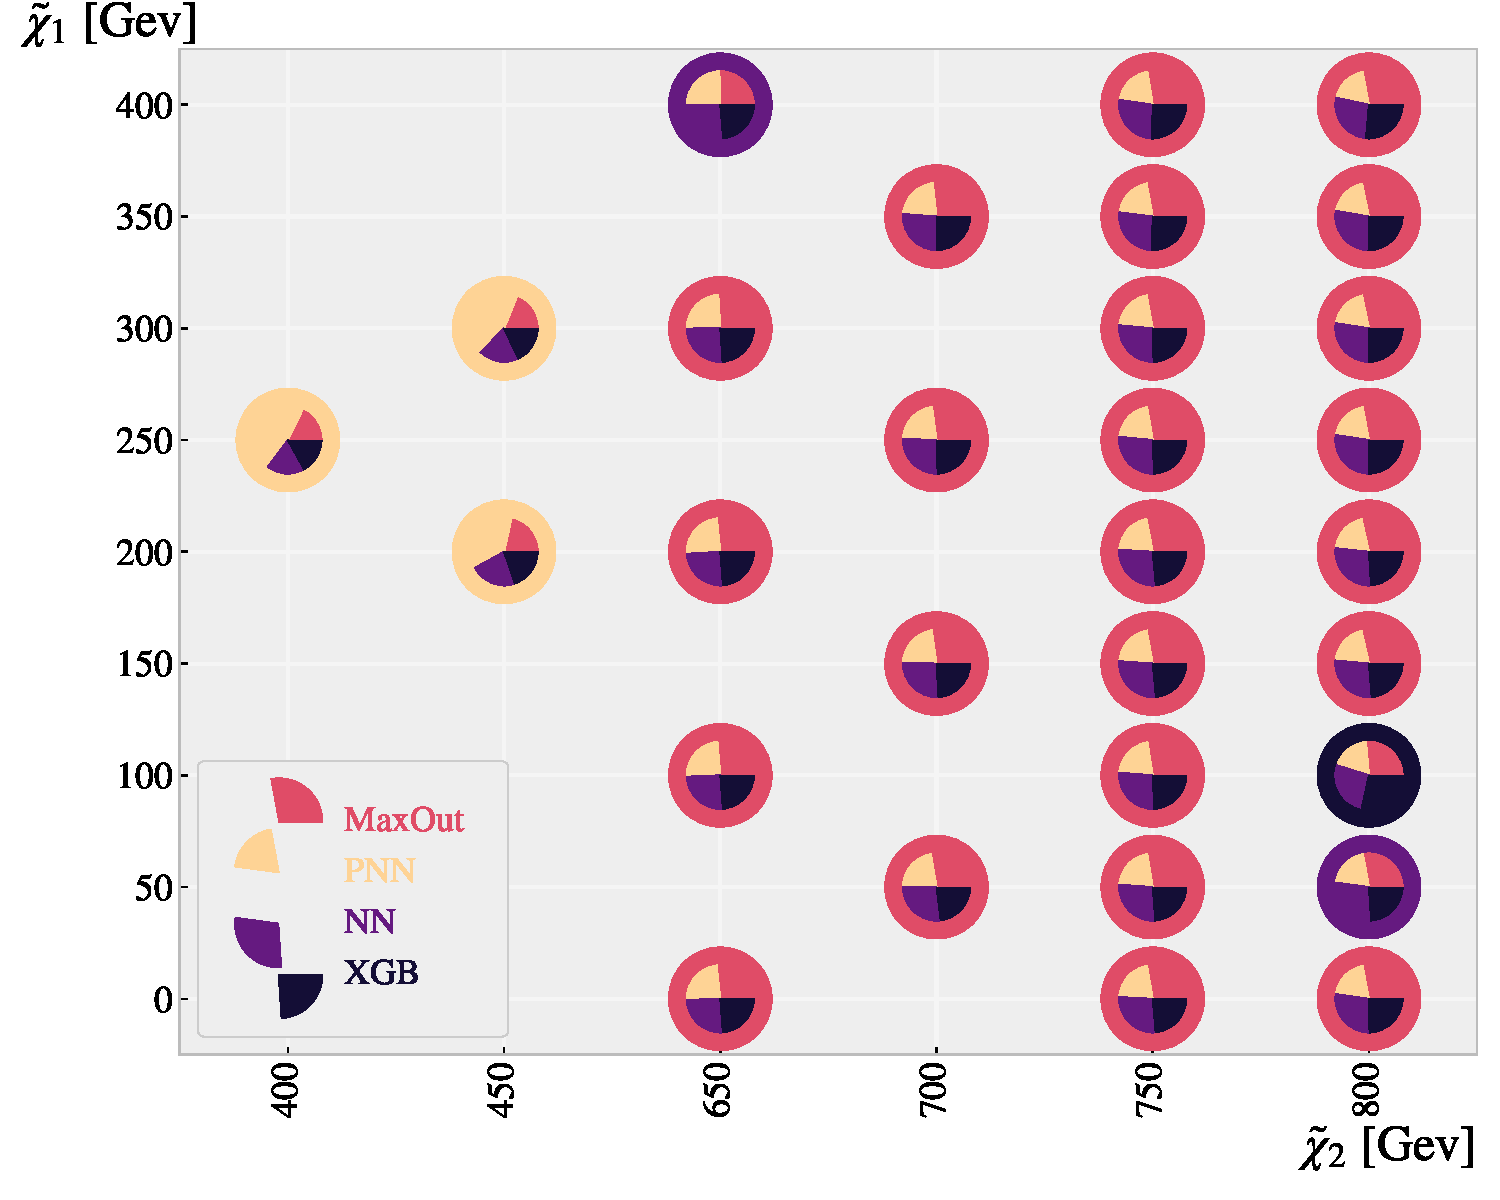
\includegraphics[width=\textwidth]{Figures/MLResults/NN/SUSY/Comparison/GenPlussXGBNetworkComp.pdf}
    \end{subfigure}
    }
    \caption[A sensitivity comparison between a dense \acs{NN}, \acs{PNN}, maxout and XGBoost on the original 
    signal data.]{A sensitivity comparison between a dense \ac{NN}, \ac{PNN}, maxout and XGBoost on the original 
    signal data. The size of each slice' represents the relative size of the significance and the color around each 
    point displays the method with the largest sensitivity for the respective combination.}
    \label{fig:GenPlussXGB}
\end{figure}
